\subsection{\centering Amicus Curiae Briefs}


\begin{figure}[H]
\centering
\caption{Average Number of Amici Filed for Granted Petitions (OT18-OT23)}
\vspace{1.5mm}
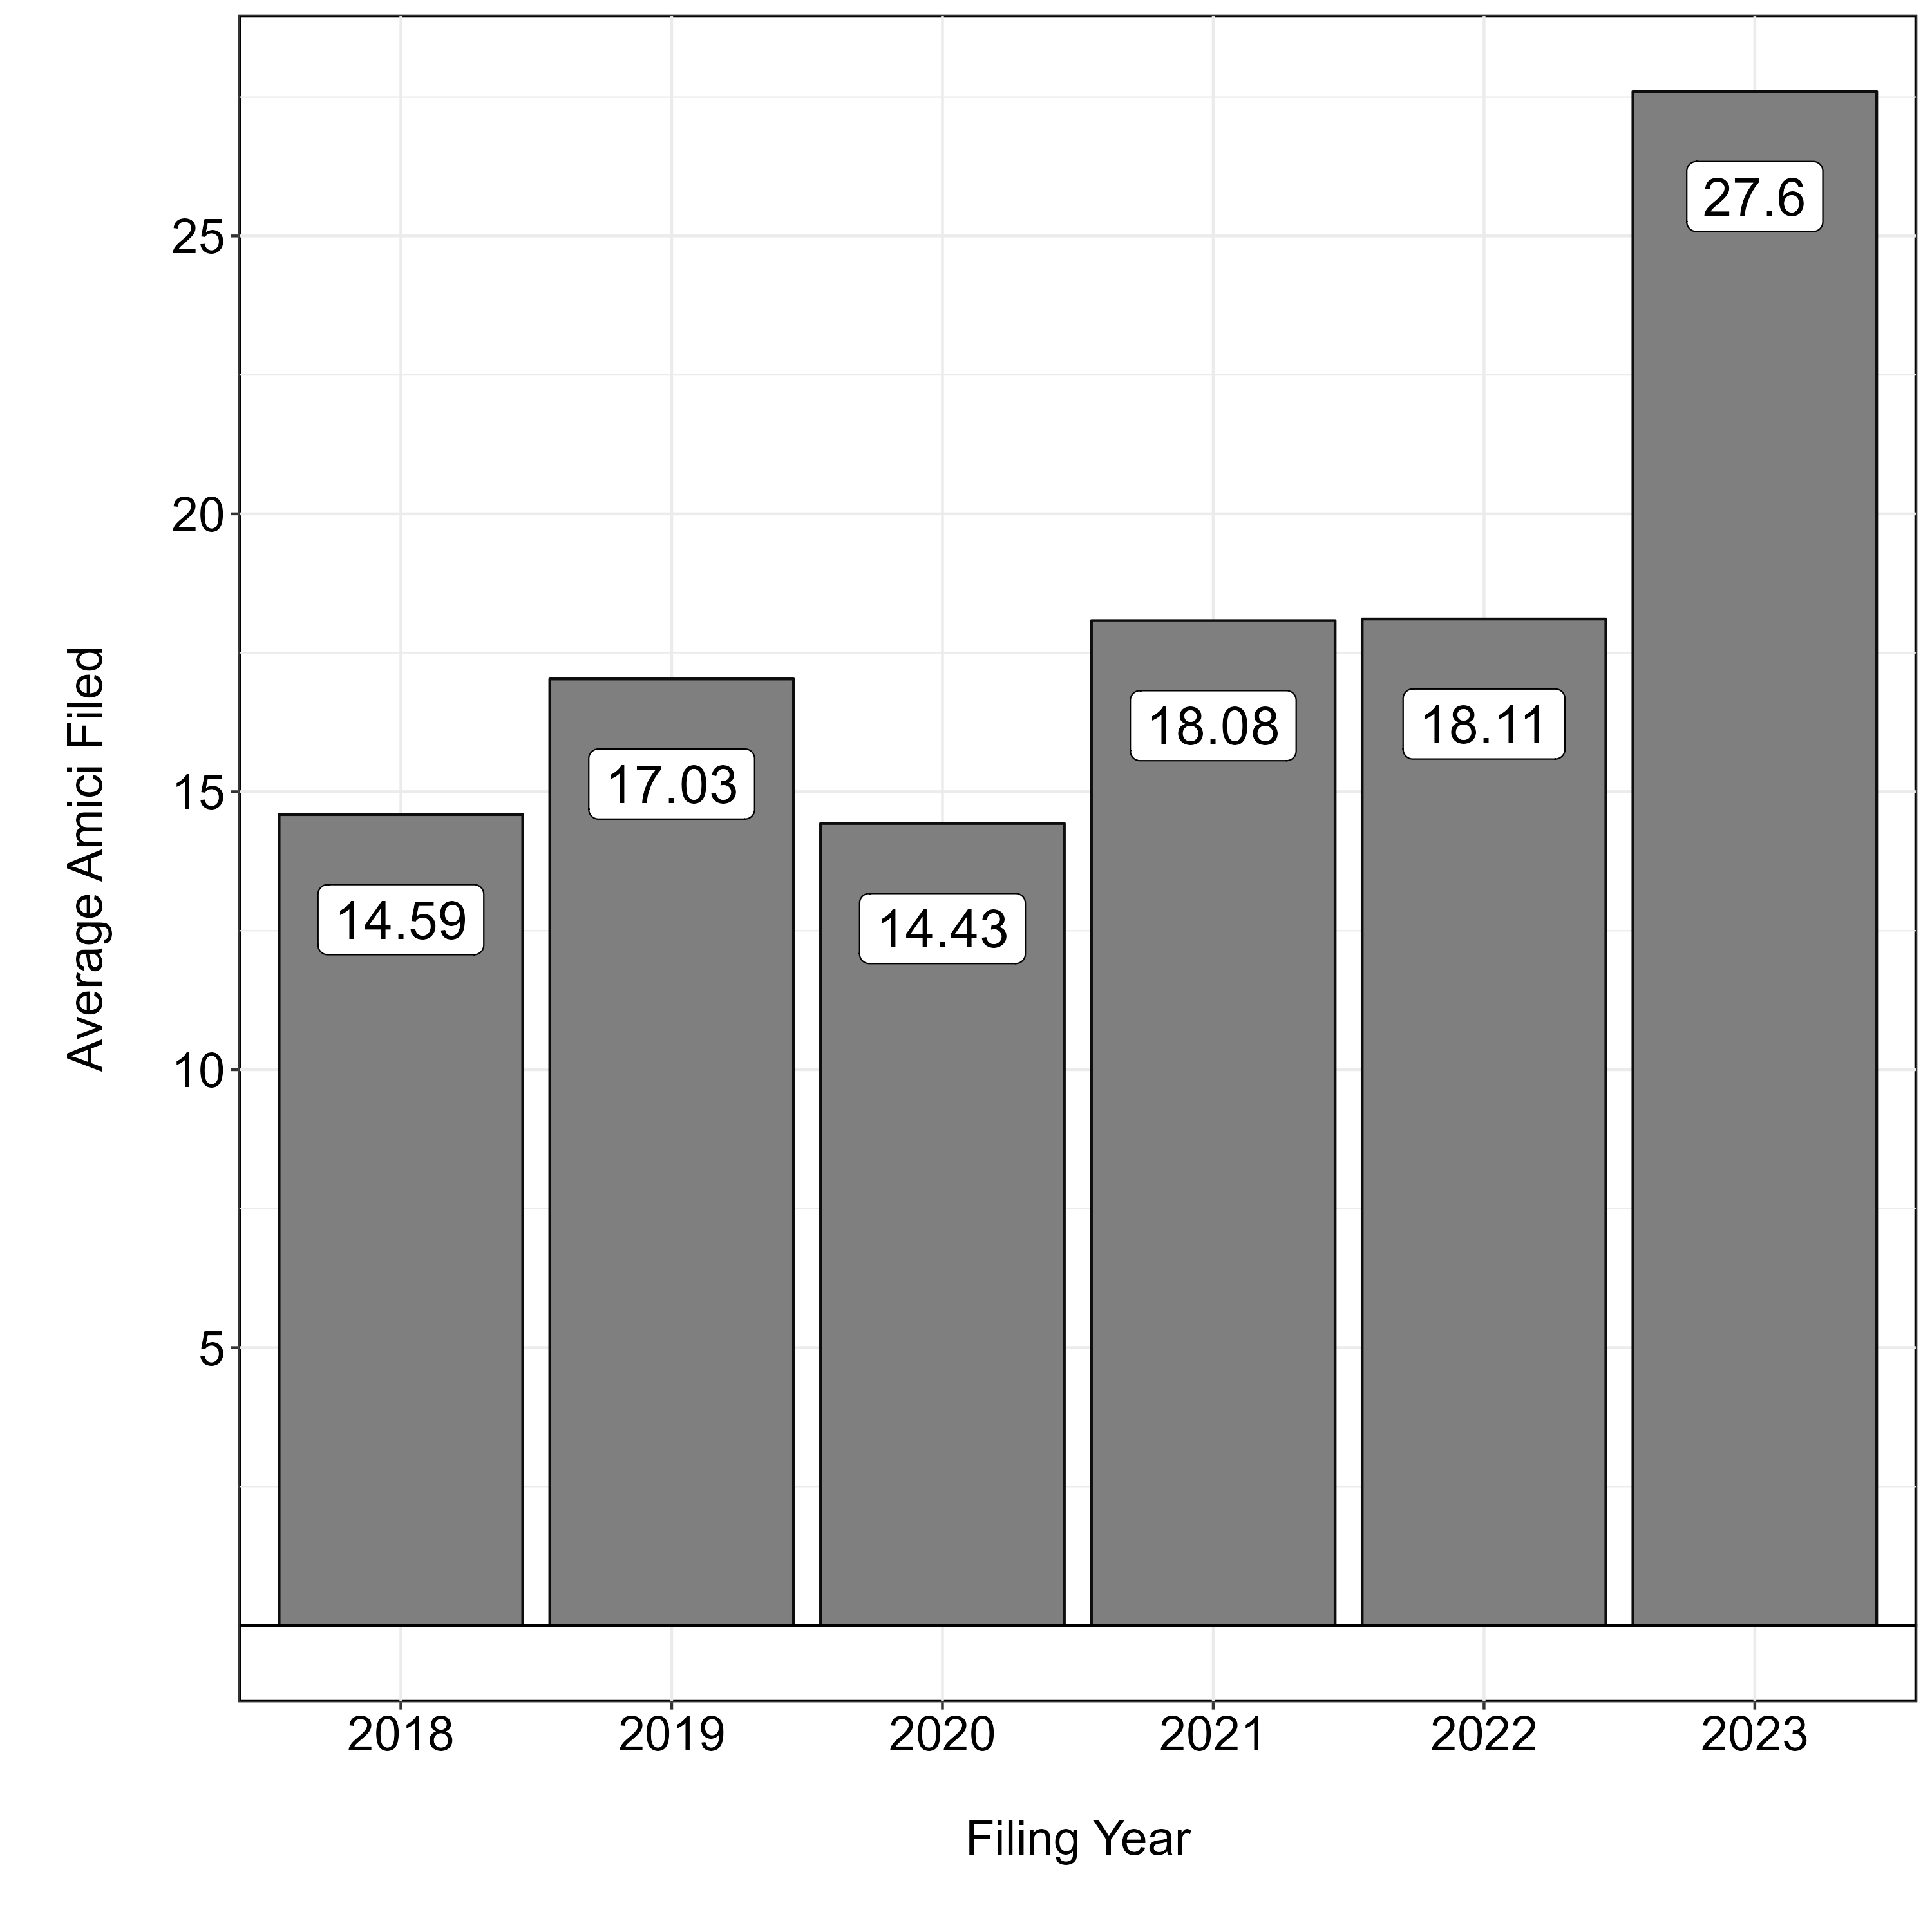
\includegraphics[width = 0.7\textwidth]{"Figures/statpack_figures/average_amici_filed_by_granted_type_granted.png"}
\end{figure}

\raggedright{
\footnotesize{\emph{Note:} Average number of amici filed considers amici filed at any (both) certiorari and granted stages. \\
\vspace{2.5mm}
\emph{Furthermore}, the x-axis (\emph{Filing Year}) represents the term when the petition was filed -- \textbf{not} when it was granted review. For example, \emph{Acheson Hotels, LLC v. Laufer} (No. 22-429) was filed during the 2022 term but was argued this term (OT2023). As such, it would be included in the bar referencing the 2022 filing year. \\
\vspace{2.5mm}
\emph{Furthermore}, given that many cases filed in OT2023 have yet to be granted (denied) review or distributed for Conference, that bar should be viewed as a preliminary diagnostic with incomplete data. \\
\vspace{2.5mm}
\emph{Finally}, Granted (Denied) does not mean the case was orally argued. For example, \emph{Danco Laboratories, LLC v. Alliance for Hippocratic Medicine} (No. 23-236) was granted and subsequently consolidated with \emph{FDA v. Alliance for Hippocratic Medicine} (No. 23-235). Although \emph{FDA} will be the recorded decision, the certiorari-stage (i.e., pre-grant stage) amici filed in \emph{Danco Laboratories} are included in the counts used to derive the average filings for the 2023 Filing Year.}}

\newpage

\begin{figure}[H]
\centering
\caption{Average Number of Amici Filed in Argued Cases (OT23)}
\vspace{1.5mm}
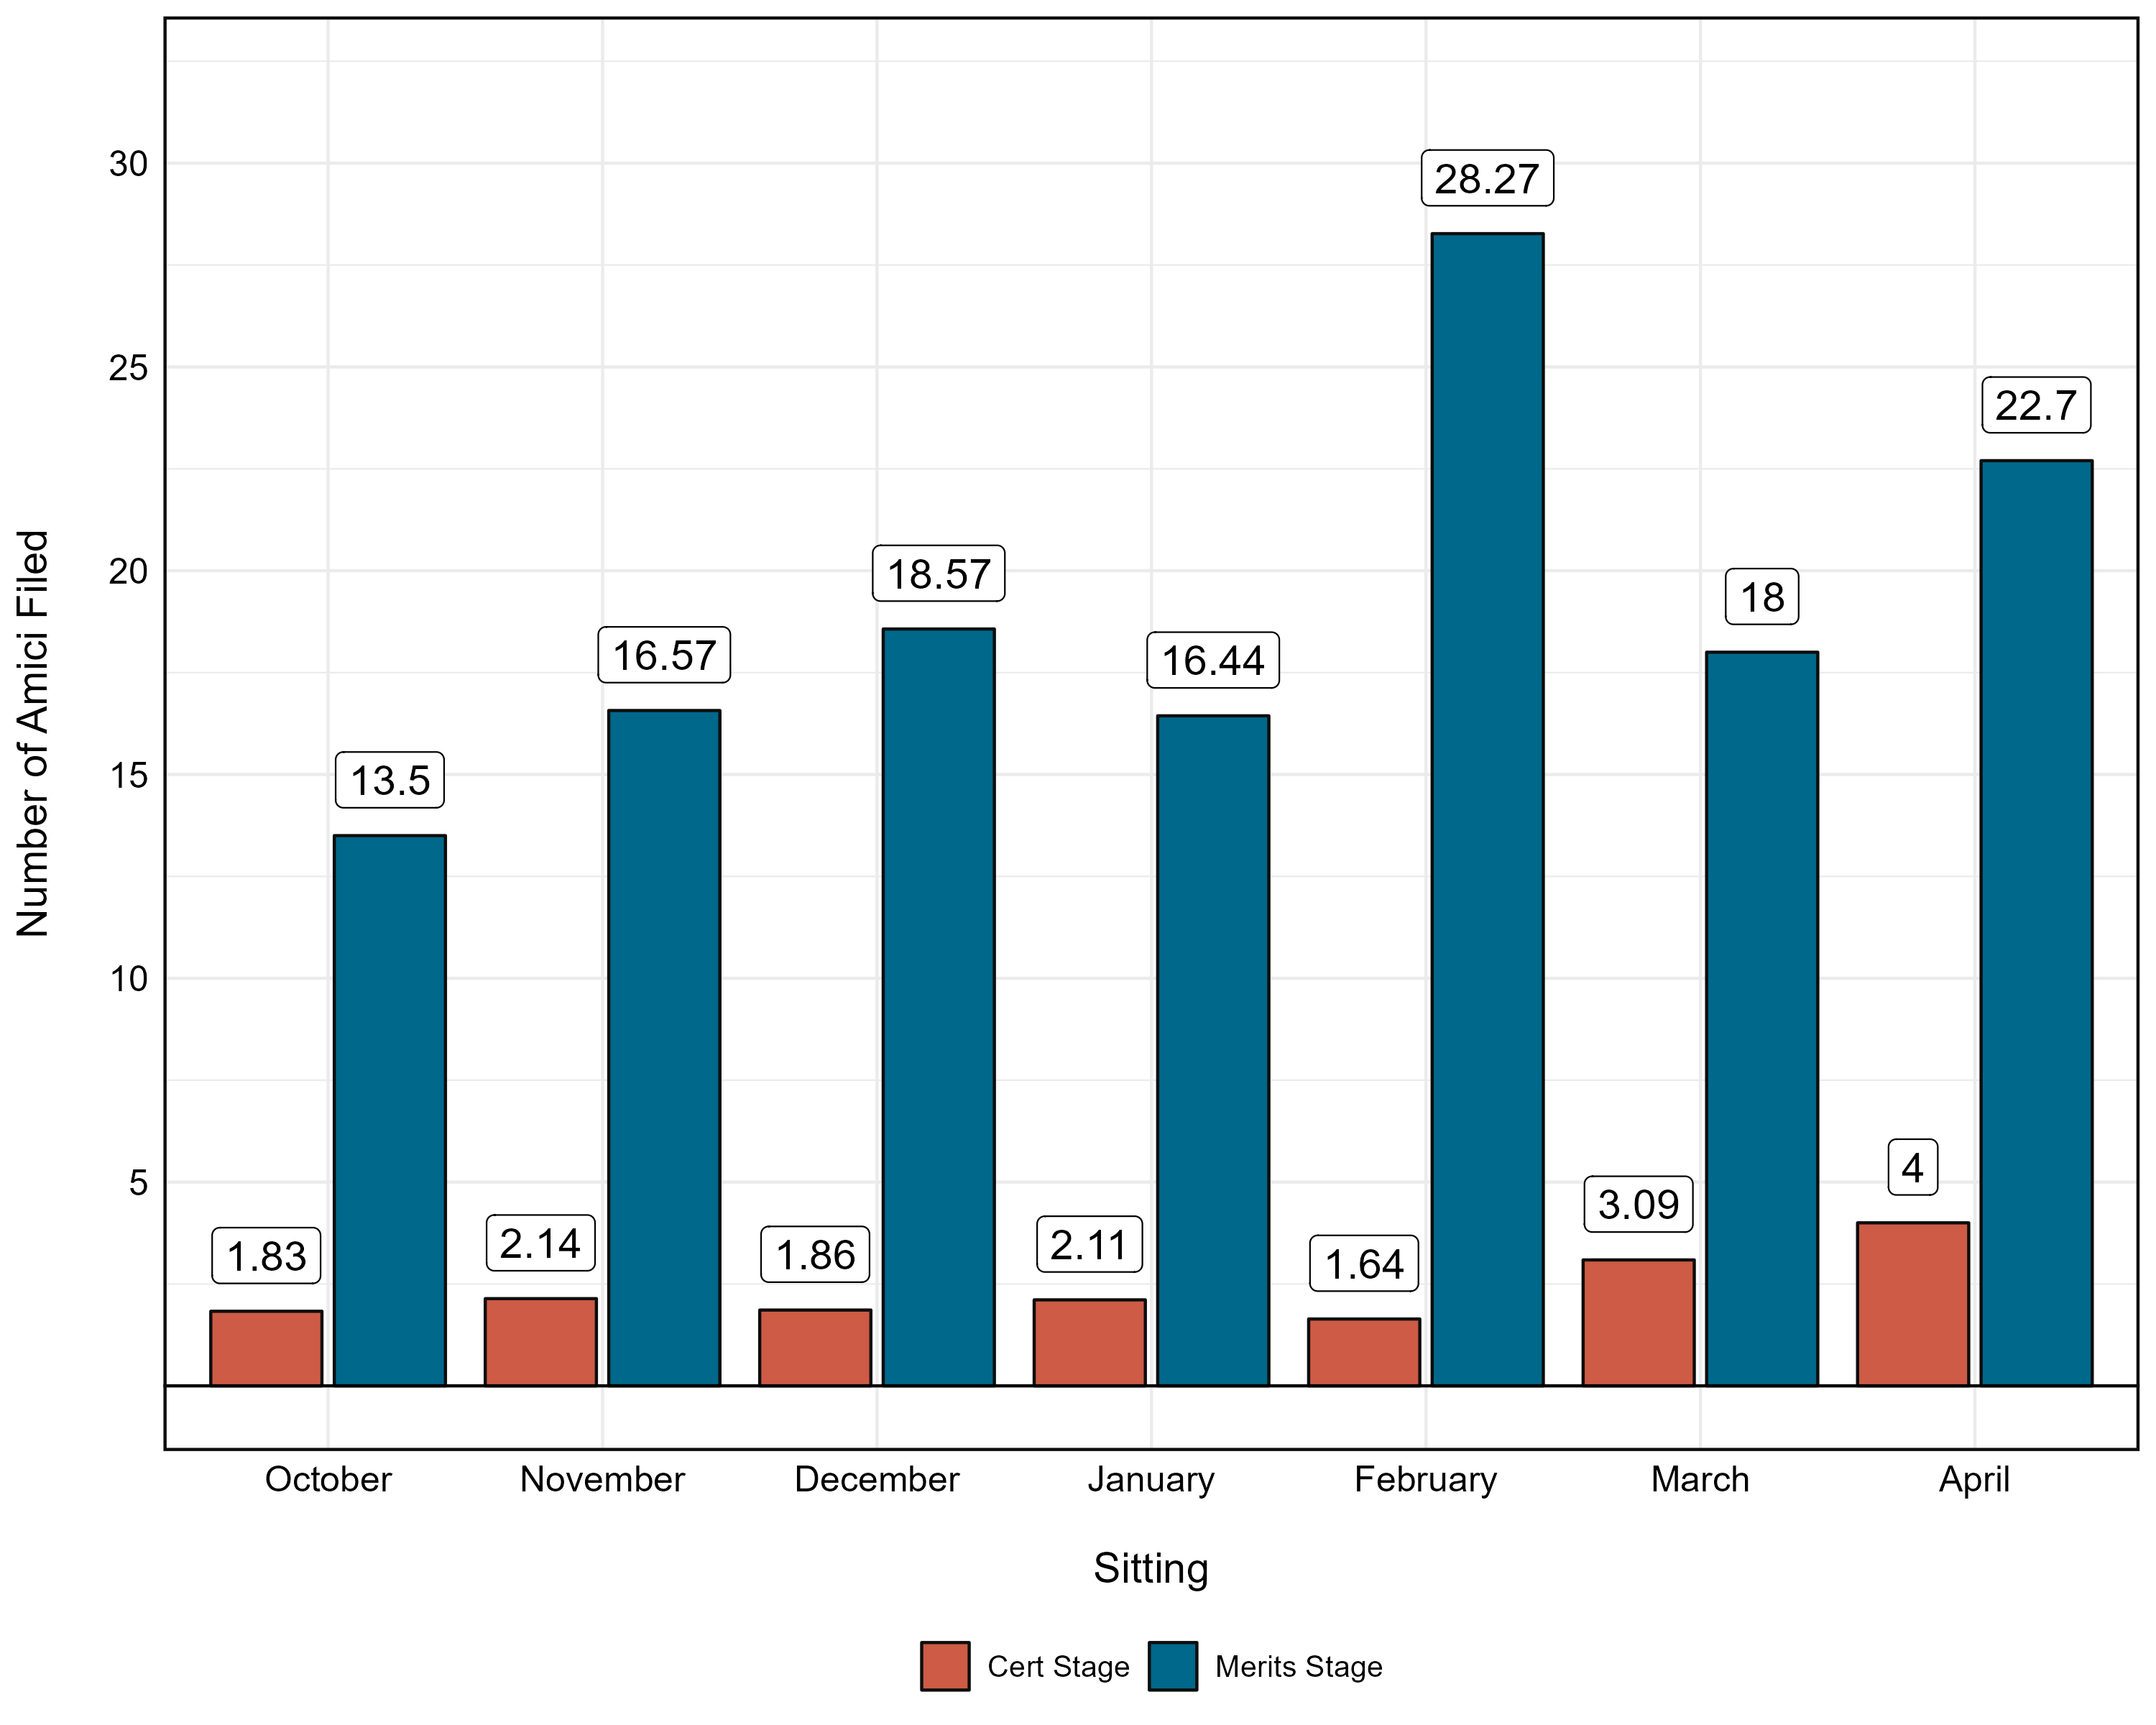
\includegraphics[width = 0.8\textwidth]{"Figures/statpack_figures/cert_merits_amici_OT23.png"}
\end{figure}

\raggedright{
\footnotesize{\emph{Note:} x-axis represents sitting when case was argued -- Ex: November Sitting (November 27, 2023 - December 6, 2023). For a case-level breakdown, please visit \href{https://empiricalscotus.com/2023-stats/}{EmpiricalSCOTUS}.}

